%%%%%%%%%%%%%%%%%%%%%%%%%%%%%%%%%%%%%%%%%
% Short Sectioned Assignment
% LaTeX Template
% Version 1.0 (5/5/12)

%
% This template has been downloaded from:
% http://www.LaTeXTemplates.com
%
% Original author:
% Frits Wenneker (http://www.howtotex.com)
%
% License:
% CC BY-NC-SA 3.0 (http://creativecommons.org/licenses/by-nc-sa/3.0/)
%
%%%%%%%%%%%%%%%%%%%%%%%%%%%%%%%%%%%%%%%%%

%----------------------------------------------------------------------------------------
%	PACKAGES AND OTHER DOCUMENT CONFIGURATIONS
%----------------------------------------------------------------------------------------

\documentclass[paper=a4, fontsize=11pt]{scrartcl} % A4 paper and 11pt font size

\usepackage{graphicx} 
\usepackage{listings}
\usepackage[T1]{fontenc} % Use 8-bit encoding that has 256 glyphs
\usepackage{fourier} % Use the Adobe Utopia font for the document - comment this line to return to the LaTeX default
\usepackage[english]{babel} % English language/hyphenation
\usepackage{amsmath,amsfonts,amsthm} % Math packages
\usepackage{caption}
\captionsetup{font = {scriptsize}}
\usepackage{lipsum} % Used for inserting dummy 'Lorem ipsum' text into the template
\usepackage{subfigure}
\usepackage{latexsym}
\usepackage{sectsty} % Allows customizing section commands
\allsectionsfont{\centering \normalfont\scshape} % Make all sections centered, the default font and small caps
\usepackage{color} %red, green, blue, yellow, cyan, magenta, black, white
\definecolor{mygreen}{rgb}{0,0.6,0}
\definecolor{mygray}{rgb}{0.5,0.5,0.5}
\definecolor{mymauve}{rgb}{0.58,0,0.82}
\usepackage{float}
\usepackage{fancyhdr} % Custom headers and footers
\pagestyle{fancyplain} % Makes all pages in the document conform to the custom headers and footers
\fancyhead{} % No page header - if you want one, create it in the same way as the footers below
\fancyfoot[L]{} % Empty left footer
\fancyfoot[C]{} % Empty center footer
\fancyfoot[R]{\thepage} % Page numbering for right footer
\renewcommand{\headrulewidth}{0pt} % Remo\label{\label{key}}ve header underlines
\renewcommand{\footrulewidth}{0pt} % Remove footer underlines
\setlength{\headheight}{13.6pt} % Customize the height of the header

\numberwithin{equation}{section} % Number equations within sections (i.e. 1.1, 1.2, 2.1, 2.2 instead of 1, 2, 3, 4)
\numberwithin{figure}{section} % Number figures within sections (i.e. 1.1, 1.2, 2.1, 2.2 instead of 1, 2, 3, 4)
\numberwithin{table}{section} % Number tables within sections (i.e. 1.1, 1.2, 2.1, 2.2 instead of 1, 2, 3, 4)
\newcommand{\mygamma}{\ensuremath{\gamma{}}}
\setlength\parindent{0pt} % Removes all indentation from paragraphs - comment this line for an assignment with lots of text

%----------------------------------------------------------------------------------------
%	TITLE SECTION
%----------------------------------------------------------------------------------------

\newcommand{\horrule}[1]{\rule{\linewidth}{#1}} % Create horizontal rule command with 1 argument of height

\title{	
\normalfont \normalsize 
\textsc{Purdue University} \\ [25pt] % Your university, school and/or department name(s)
\horrule{0.5pt} \\[0.4cm] % Thin top horizontal rule
\huge ECE 637 Laboratory Exercise 7 \\ 
\huge Image Restoration\\% The assignment title
\horrule{2pt} \\[0.5cm] % Thick bottom horizontal rule
}

\author{Tong Shen} % Your name

\date{\normalsize\today} % Today's date or a custom date

\begin{document}

\maketitle % Print the title

%----------------------------------------------------------------------------------------
%	PROBLEM 1
%----------------------------------------------------------------------------------------
\section{Minimum Mean Square Error (MMSE) Linear Filters
}

Often filters are designed to minimize the mean squared error between a desired image and
the available noisy or distorted image. When the filter is linear, minimum mean squared
error (MMSE) filters may be designed using closed form matrix expressions.
\vspace{10in}
\\

For the report, this is the four original images. 
\begin{figure}[H]
	
	\centering
	\subfigure[\emph{img14g.tif}]{
		
		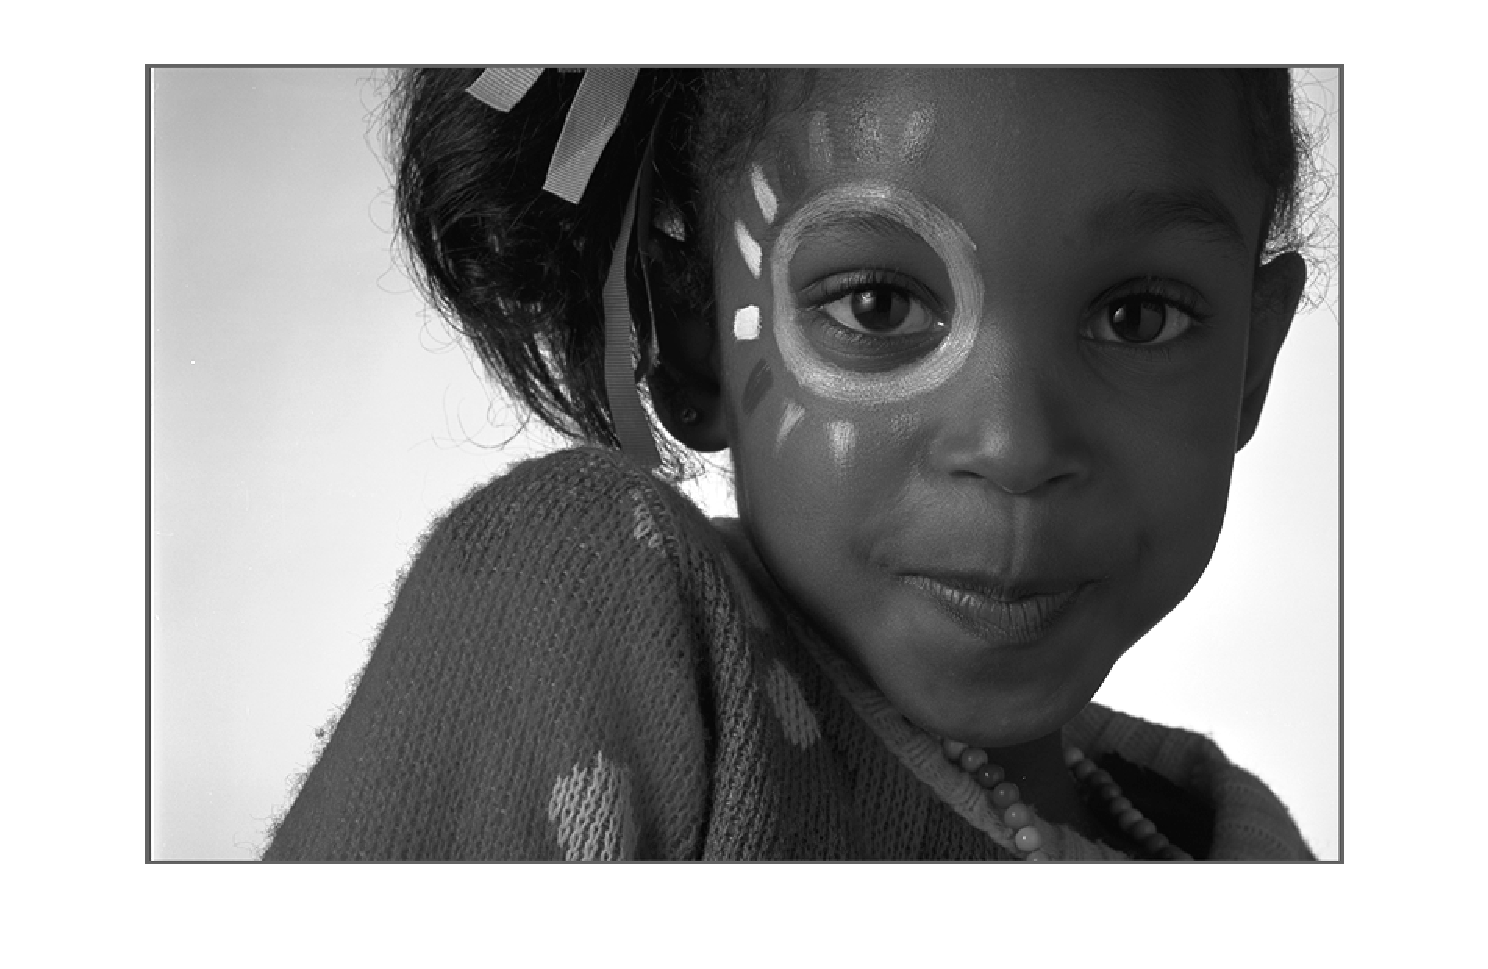
\includegraphics[width=2.5in]{g.eps}}
\hspace{0in} 
	\subfigure[\emph{img14bl.tif}]{
		
		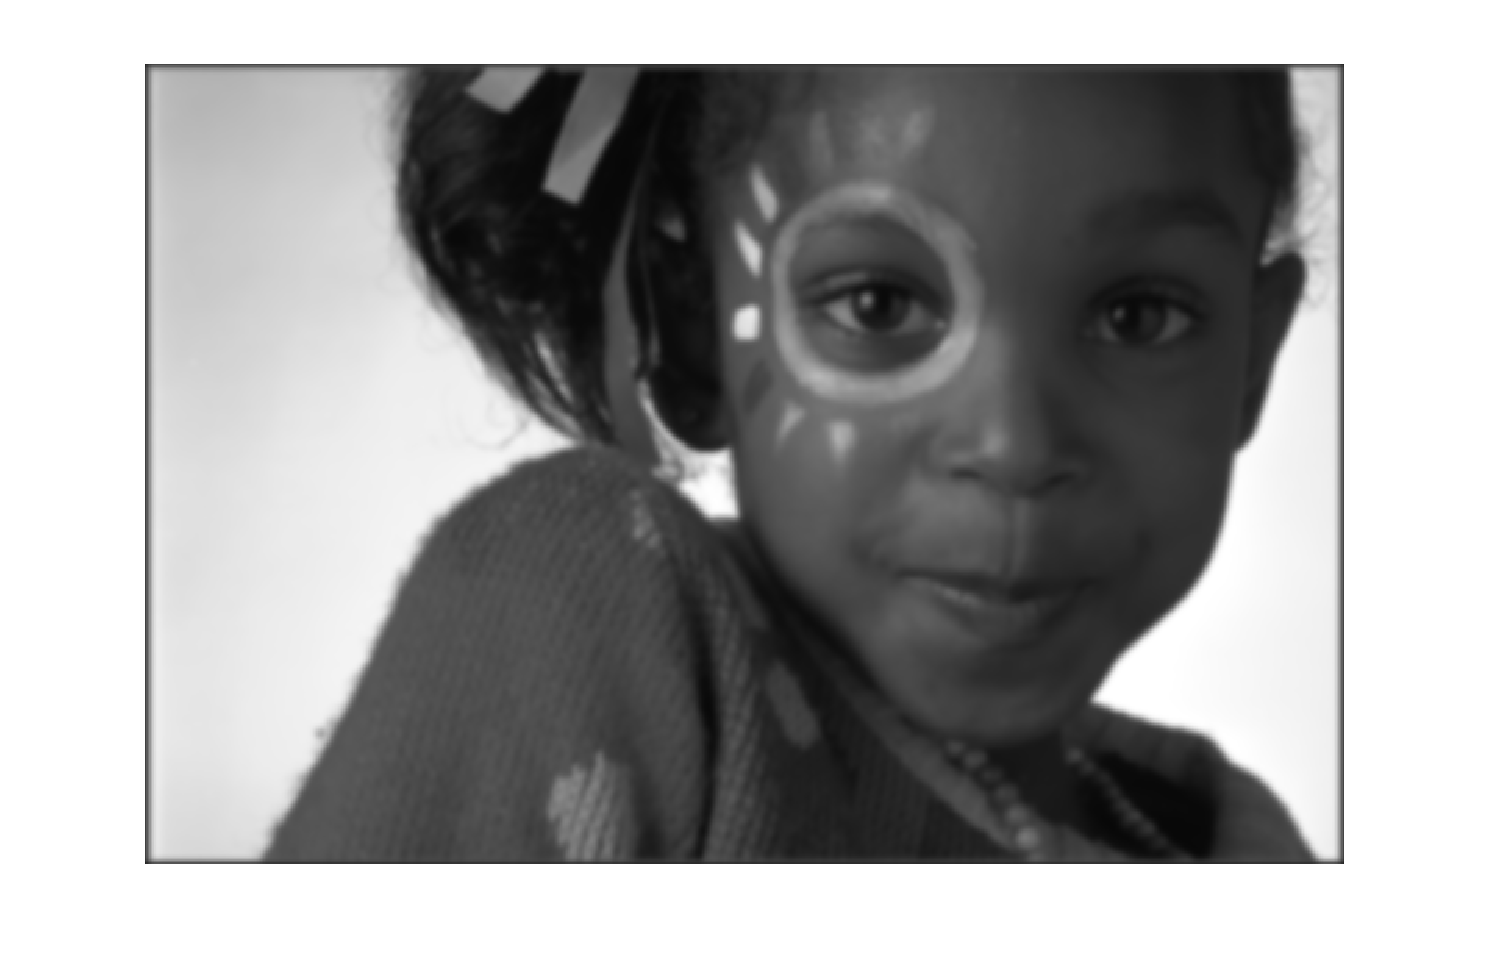
\includegraphics[width=2.5in]{bl.eps}}
\hspace{0in} 
	\subfigure[\emph{img14sp.tif}]{
		
		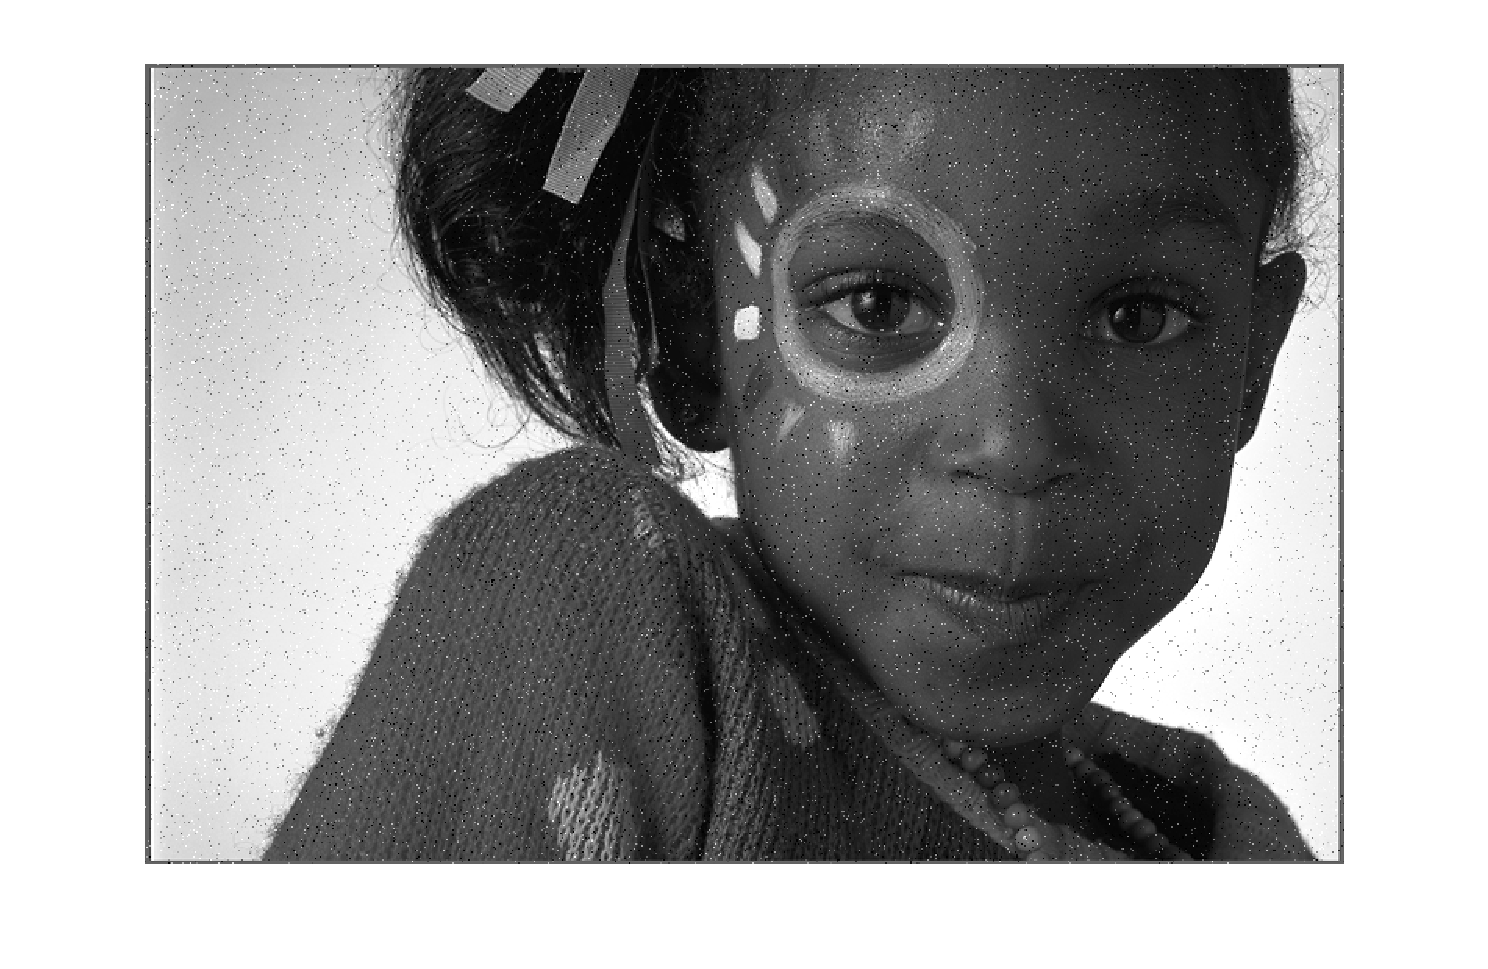
\includegraphics[width=2.5in]{sp.eps}}
	\hspace{0in} 
	\subfigure[\emph{img14gn.tif}]{
		
		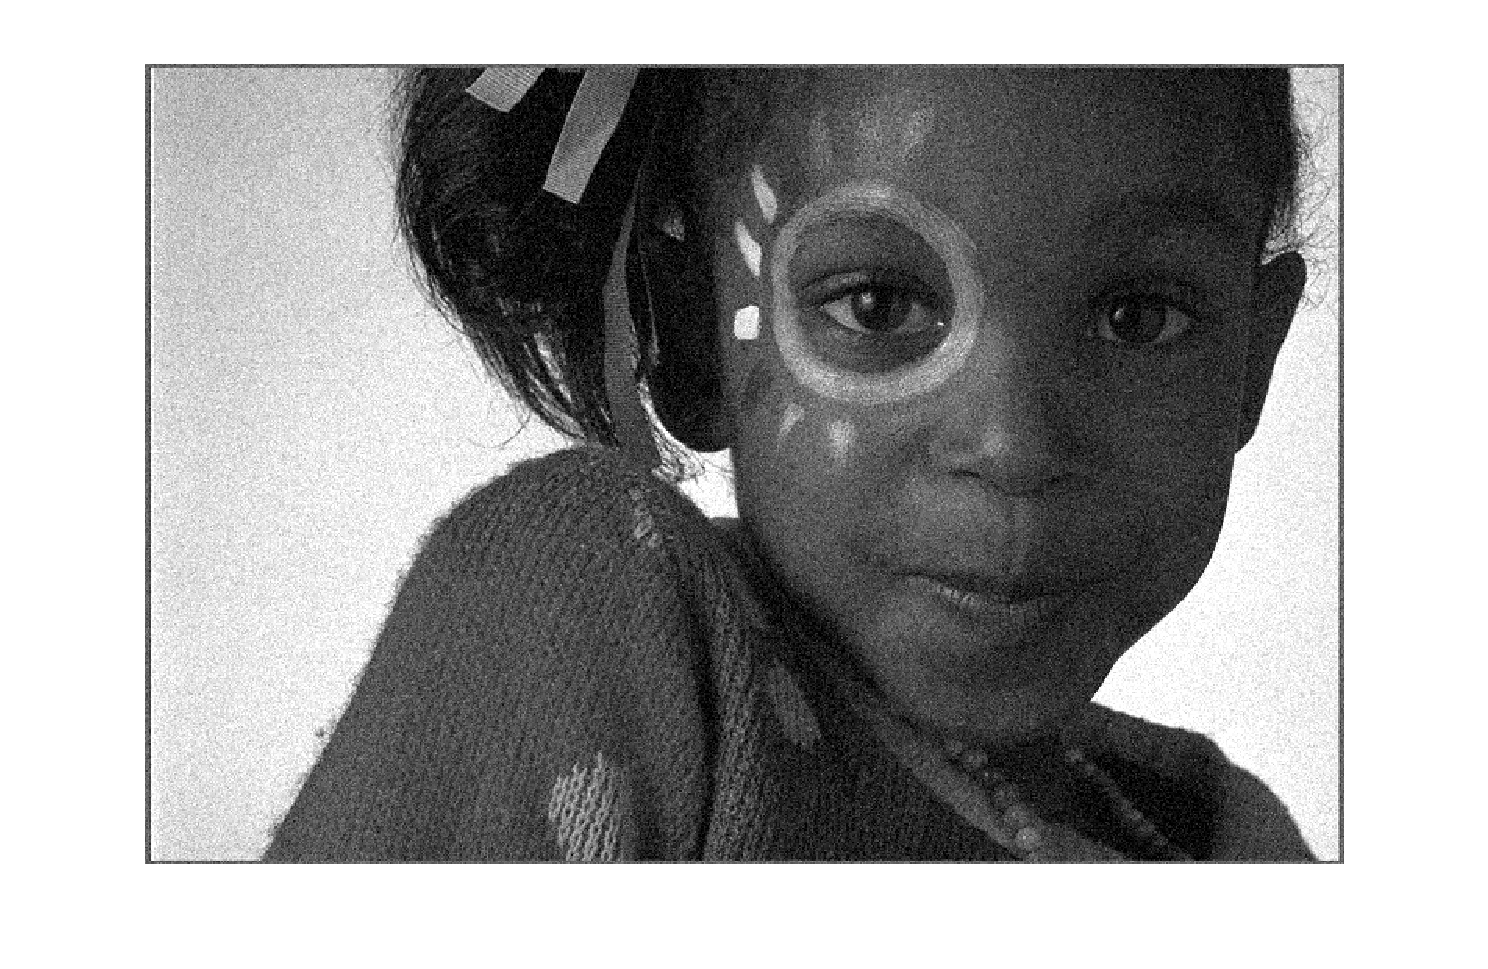
\includegraphics[width=2.5in]{gn.eps}}
	\caption{The four original images}
	
\end{figure}
\vspace{10in}


And the optimal filtered images are as follows:
 
\begin{figure}[H]
	
	\centering
	\subfigure[ optimal filtered blurred images]{
		
		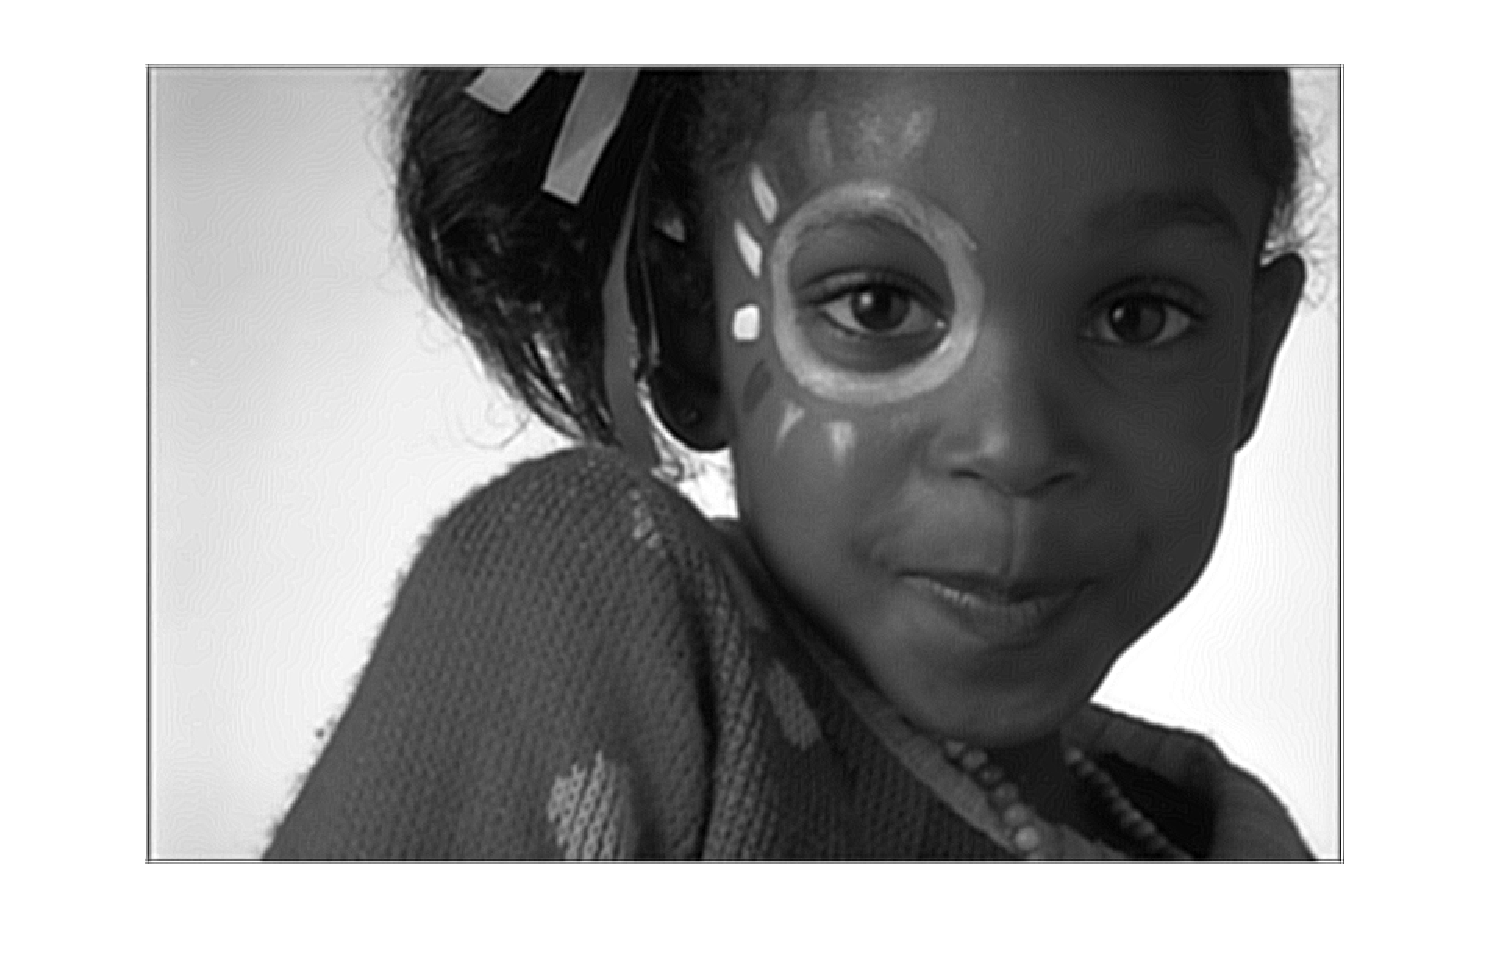
\includegraphics[width=2.5in]{blf.eps}}
	\hspace{1in}
	\subfigure[ optimal filtered noisy images]{
		
		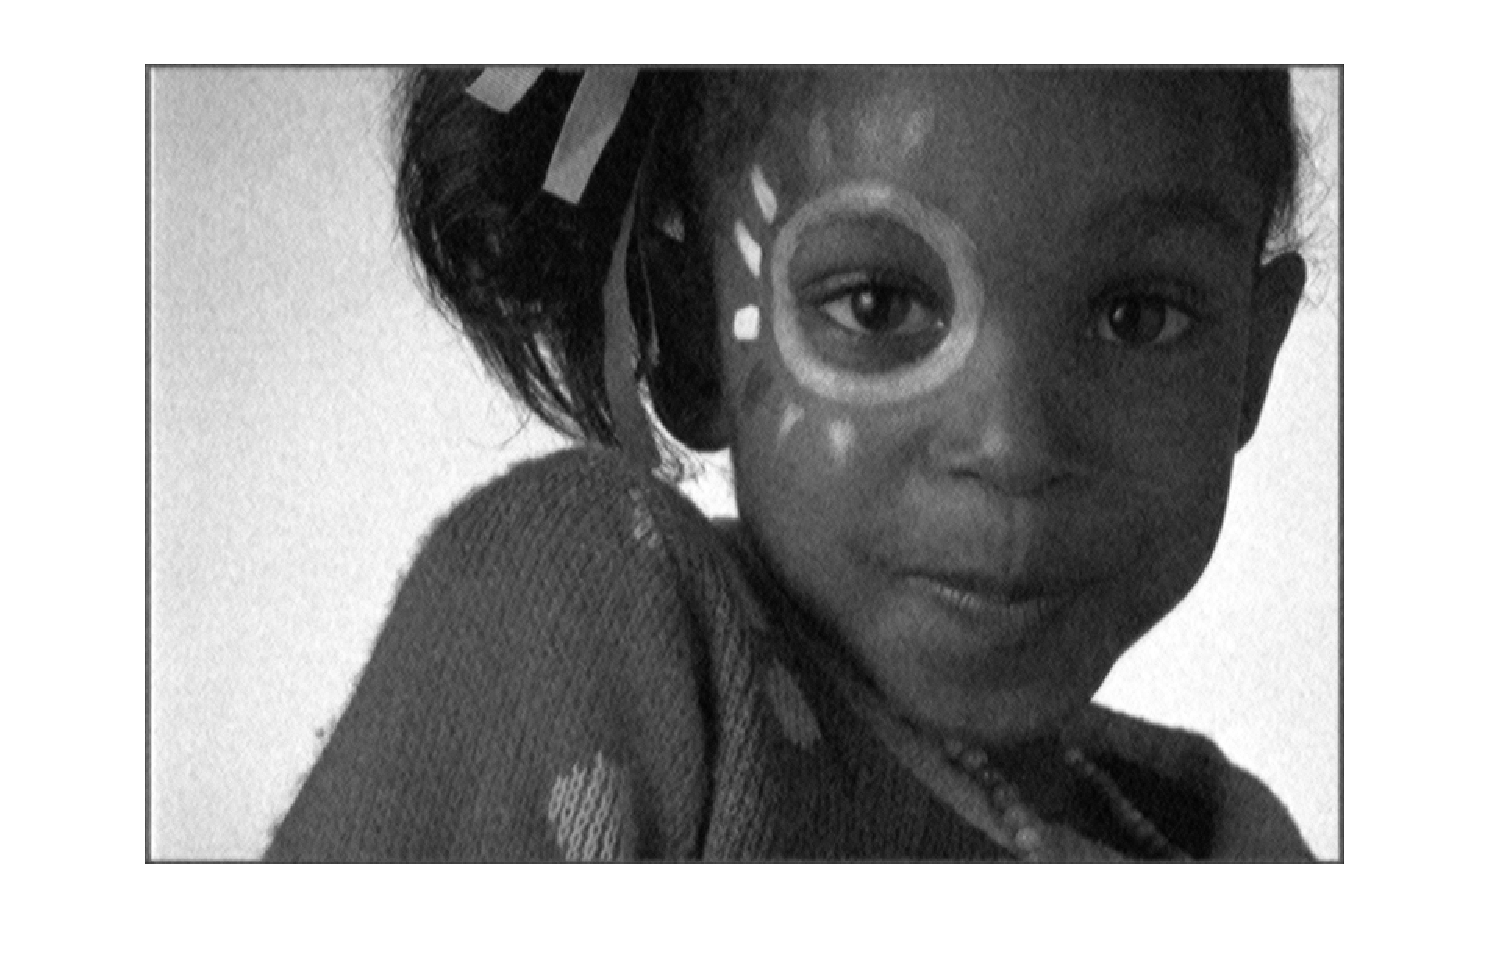
\includegraphics[width=2.5in]{gnf.eps}}
	\subfigure[ optimal filtered spotted noisy images]{
		
		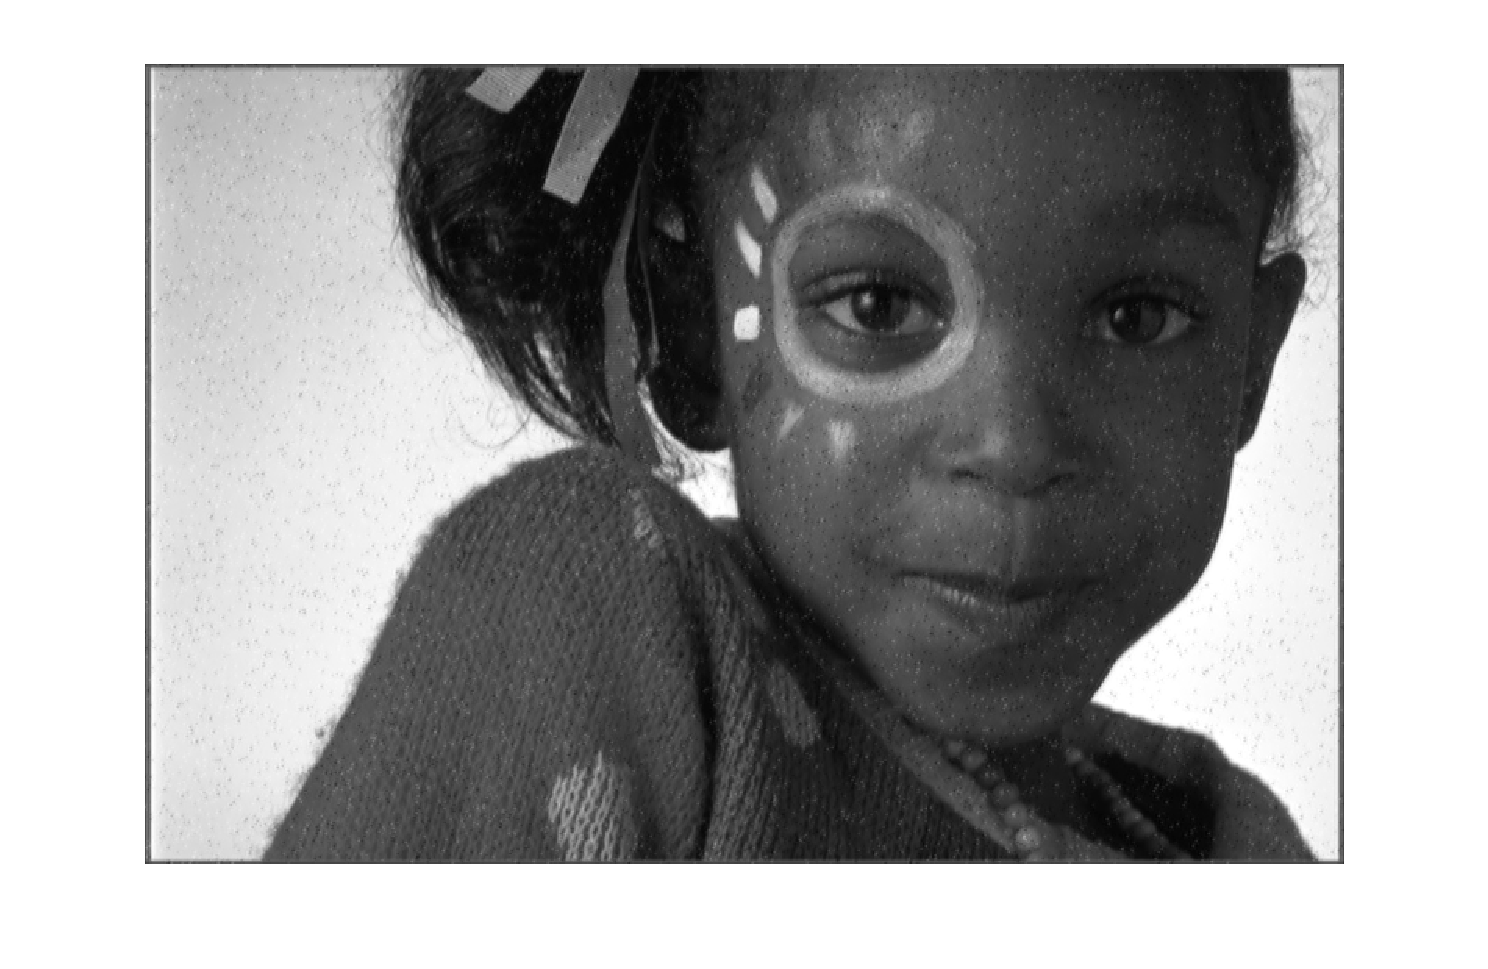
\includegraphics[width=2.5in]{spf.eps}}

	\caption{ Optimal filtered images}
	
\end{figure}

And for the blurred image, the  optimal filtering matrix is: 

\[
\theta^{\star} = 
\begin{bmatrix}
   0.3720   & 0.2052   &-0.9682   & 1.0572 &0.1961   &-1.0020    &0.9254 \\
-0.0431    &0.4069  & -1.2219 &  -0.0280 &-0.6146  & -1.3229    &0.4024\\
-0.3541   &-0.3242   &-0.4810   & 0.3321 &0.7580  & -0.0871   &-0.7923\\
1.1089   &-2.4308    &1.9317   & 3.7782 &1.5691  & -0.0701    &0.0615\\
0.3791   &-0.4590  & -1.1045  &  1.2263& 0.8358  & -1.4710    &0.3905\\
-1.0990   &-0.1802  & -0.2944  &  1.0624 &-1.8928   &-1.9628    &0.8127\\
1.1560    &0.4776   &-1.7439  &  0.6483 &0.2949   & 0.2604   & 0.3042




\end{bmatrix}
\]

For the noisy image, the optimal filtering matrix is: 

\[
\theta^{\star} = 
\begin{bmatrix}
0.0165  &  0.0259   & 0.0044  &  0.0050  & -0.0080   & 0.0302   &-0.0259\\

-0.0055  &  0.0053  &  0.0355  &  0.0205 &0.0464   & 0.0091  &  0.0066\\

-0.0105  & -0.0125   & 0.0674  &  0.0731& 0.0470  &  0.0290  & -0.0030\\

-0.0091  & -0.0153  &  0.0476  &  0.2306 &0.0891  & -0.0175  &  0.0011\\

-0.0050  & -0.0222  &  0.0423   & 0.1117 &0.0650  & -0.0118 &   0.0069\\

-0.0044   & 0.0079  &  0.0307  &  0.0268& 0.0088  & -0.0063  &  0.0192\\

-0.0053  & -0.0043  &  0.0154  &  0.0127 & 0.0140 &   0.0183    &0.0054



\end{bmatrix}
\]
For the spotted noisy image, the optimal filtering matrix is: 
\[
\theta^{\star} = 
\begin{bmatrix}
    0.0080   & 0.0048  & -0.0016 &  -0.0050 &0.0257   &-0.0209   &-0.0185\\

0.0017  & -0.0016   & 0.0558  &  0.0267     &0.0435  &  0.0214  &  0.0196\\

-0.0010  &  0.0042  &  0.0413   & 0.0968& 0.0212 &  -0.0196   & 0.0199\\

-0.0014 &  -0.0203  &  0.0350  &  0.2652& 0.1492  & -0.0287   & 0.0083\\

0.0252   & 0.0023   & 0.0612   & 0.0965 &0.0154   &-0.0412  &  0.0233\\

-0.0099  & -0.0006  &  0.0313  &  0.0497 &0.0143  &  0.0038   & 0.0131\\

-0.0407   & 0.0162  & -0.0068  &  0.0100& 0.0079   & 0.0129 &  -0.0110


\end{bmatrix}
\]

\section{Weighted Median Filtering}
A simple median filter is a nonlinear filter which simply replaces each pixel with the
median from a set in a window surrounding the pixel. It has the effect of minimizing the
absolute prediction error.

\\
\vspace{0.2in}
The follow two image is the filtered result using the median filter:
\begin{figure}[H]
	\centering
	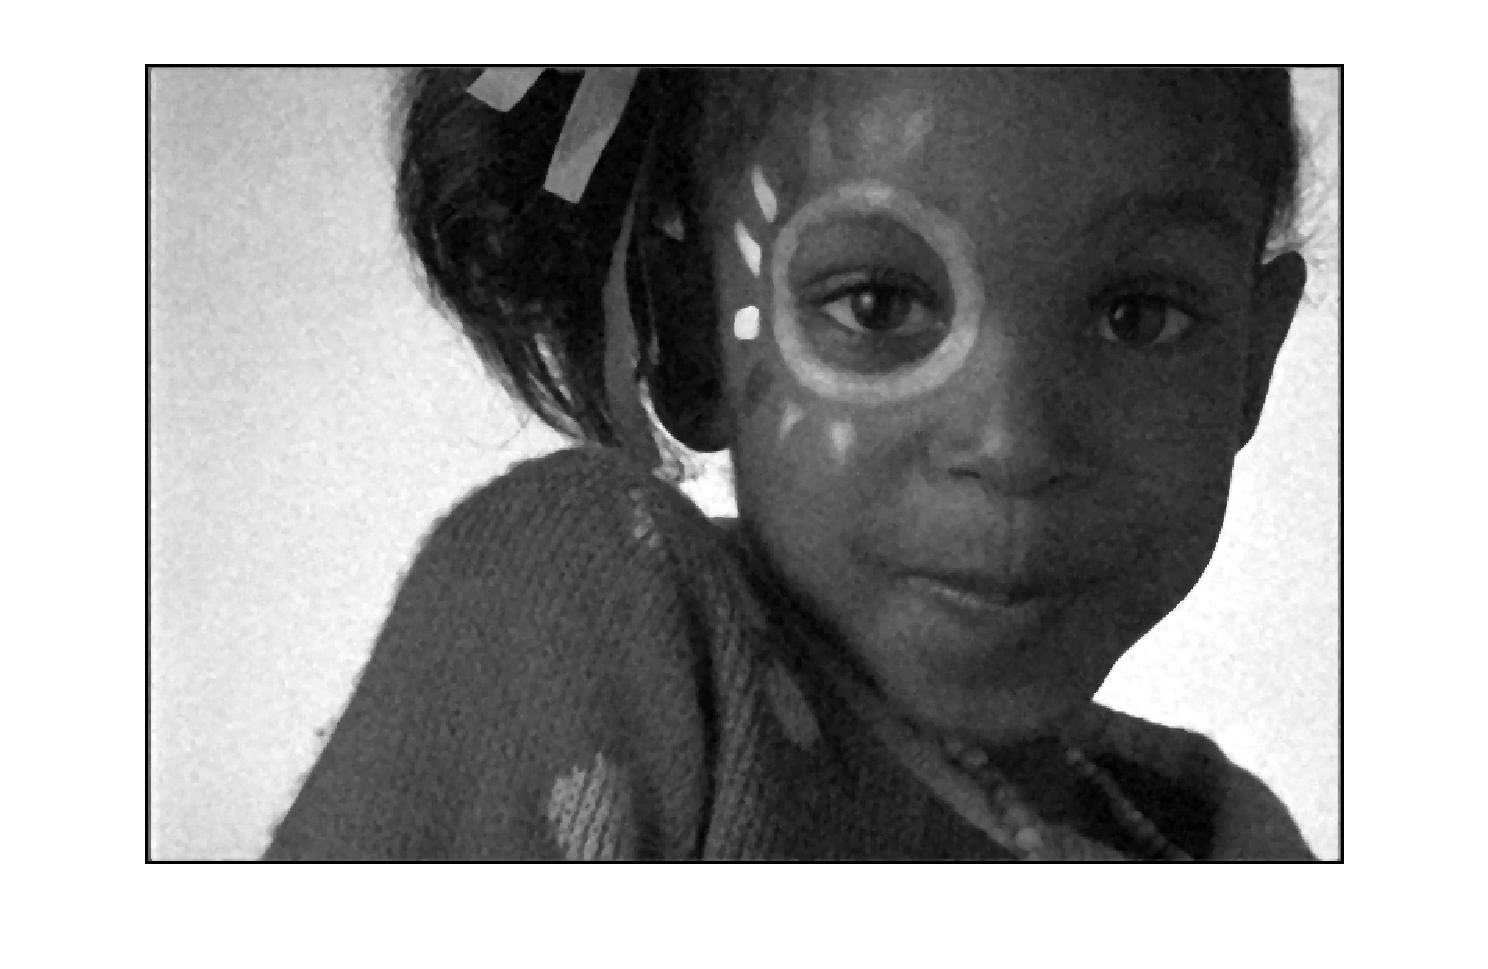
\includegraphics[height = 3in]{gnmff.eps}
	\caption{The median filtered image of \emph{img14gn.tif}}
\end{figure}

\begin{figure}[H]
	\centering
	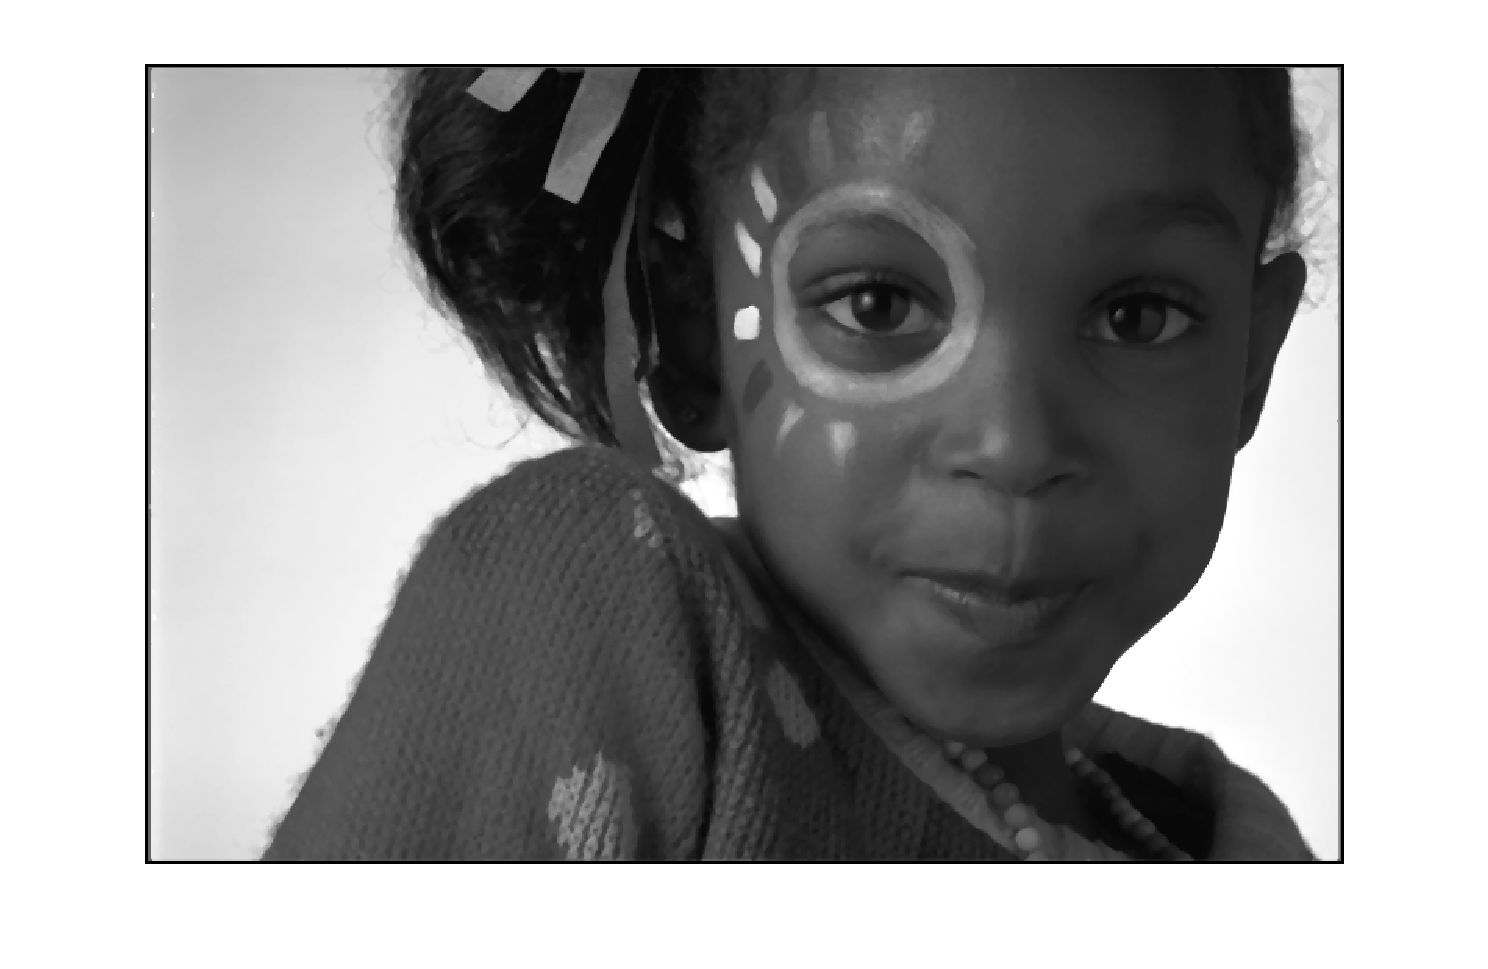
\includegraphics[height = 3in]{gnmf.eps}
	\caption{The median filtered image of \emph{img14sp.tif}}
\end{figure}


\subsection{Code listing}

\lstset{ %
	backgroundcolor=\color{white},   % choose the background color; you must add \usepackage{color} or \usepackage{xcolor}; should come as last argument
	basicstyle=\footnotesize,        % the size of the fonts that are used for the code
	breakatwhitespace=false,         % sets if automatic breaks should only happen at whitespace
	breaklines=true,                 % sets automatic line breaking
	captionpos=b,                    % sets the caption-position to bottom
	commentstyle=\color{mygreen},    % comment style
	deletekeywords={...},            % if you want to delete keywords from the given language
	escapeinside={\%*}{*)},          % if you want to add LaTeX within your code
	extendedchars=true,              % lets you use non-ASCII characters; for 8-bits encodings only, does not work with UTF-8
	frame=single,	                   % adds a frame around the code
	keepspaces=true,                 % keeps spaces in text, useful for keeping indentation of code (possibly needs columns=flexible)
	keywordstyle=\color{blue},       % keyword style
	language=Octave,                 % the language of the code
	morekeywords={*,...},           % if you want to add more keywords to the set
	numbers=left,                    % where to put the line-numbers; possible values are (none, left, right)
	numbersep=5pt,                   % how far the line-numbers are from the code
	numberstyle=\tiny\color{mygray}, % the style that is used for the line-numbers
	rulecolor=\color{black},         % if not set, the frame-color may be changed on line-breaks within not-black text (e.g. comments (green here))
	showspaces=false,                % show spaces everywhere adding particular underscores; it overrides 'showstringspaces'
	showstringspaces=false,          % underline spaces within strings only
	showtabs=false,                  % show tabs within strings adding particular underscores
	stepnumber=2,                    % the step between two line-numbers. If it's 1, each line will be numbered
	stringstyle=\color{mymauve},     % string literal style
	tabsize=2,	                   % sets default tabsize to 2 spaces
	title=\lstname                   % show the filename of files included with \lstinputlisting; also try caption instead of title
}

\begin{lstlisting}

#include <math.h>
#include "tiff.h"
#include "allocate.h"
#include "randlib.h"
#include "typeutil.h"

void error(char *name);
int filter(struct TIFF_img input, int x, int y) {
unsigned int image[25];
unsigned int filter[25] = {1,1,1,1,1,1,2,2,2,1,1,2,2,2,1,1,2,2,2,1,1,1,1,1,1 };
unsigned int temp;
unsigned int num = 0;
int location;
for (int i = x - 2; i < x + 3; i++) {
for (int j = y - 2; j < y + 3; j++) {
image[num] = input.mono[i][j];
num++;
}
}
for (int i = 0; i < 24; i++) {
int isSorted = 1;
for (int j = 0; j<24 - i; j++)
{
if (image[j] > image[j + 1])
{
isSorted = 0;
temp = image[j];
image[j] = image[j + 1];
image[j + 1] = temp;

temp = filter[j];
filter[j] = filter[j + 1];
filter[j + 1] = temp;
}
}
if (isSorted == 1) break; 
}
temp = 0;
for (int i = 0; i < 25; i++) {
temp = temp + filter[i];
if (temp >= 17) {
location = i;
break;
}
}
return image[location];
}
int main (int argc, char **argv) 
{
FILE *fp;
struct TIFF_img input_img, output_img;
double **img1,**img2;
int i,j;

if ( argc != 2 ) error( argv[0] );

/* open image file */
if ( ( fp = fopen ( argv[1], "rb" ) ) == NULL ) {
fprintf ( stderr, "cannot open file %s\n", argv[1] );
exit ( 1 );
}

/* read image */
if ( read_TIFF ( fp, &input_img ) ) {
fprintf ( stderr, "error reading file %s\n", argv[1] );
exit ( 1 );
}

/* close image file */
fclose ( fp );

/* check the type of image data */
if ( input_img.TIFF_type != 'g' ) {
fprintf ( stderr, "error:  image must be grayscale\n" );
exit ( 1 );
}

/* Allocate image of double precision floats */
img1 = (double **)get_img(input_img.width,input_img.height,sizeof(double));
img2 = (double **)get_img(input_img.width,input_img.height,sizeof(double));

/* copy image to double array */
for ( i = 0; i < input_img.height; i++ )
for ( j = 0; j < input_img.width; j++ ) {
img1[i][j] = input_img.mono[i][j];
}

/* Filter image */
for ( i = 2; i < input_img.height - 2; i++ )
for ( j = 2; j < input_img.width - 2; j++ ) {
img2[i][j] = filter(input_img, i, j);
}

/* set up structure for output image */
get_TIFF(&output_img, input_img.height, input_img.width, 'g');

/* Fill in boundary pixels */
for (i = 0; i < input_img.height; i++)
for (j = 0; j < input_img.width; j++) {
if (i<2||i>input_img.height-3||j<2||j> input_img.width - 3)
{
img2[i][j] = 0;
}
output_img.mono[i][j] = img2[i][j];
}



/* open output image file */
if ( ( fp = fopen ( "output_img.tif", "wb" ) ) == NULL ) {
fprintf ( stderr, "cannot open file green.tif\n");
exit ( 1 );
}

/* write output image */
if ( write_TIFF ( fp, &output_img ) ) {
fprintf ( stderr, "error writing TIFF file %s\n", argv[2] );
exit ( 1 );
}

/* close green image file */
fclose ( fp );

/* de-allocate space which was used for the images */
free_TIFF ( &(input_img) );
free_TIFF ( &(output_img) );

free_img( (void**)img1 );
free_img( (void**)img2 );  

return(0);
}

void error(char *name)
{
exit(1);
}


\end{lstlisting}
 

	
	
	

	


\end{document}